\documentclass[12pt]{article}
\usepackage[utf8]{inputenc}
\usepackage{graphicx}
\usepackage{geometry}
\usepackage{titlesec}
\usepackage{hyperref}
\usepackage{booktabs}
\usepackage{float}
\usepackage{parskip}
\usepackage{caption}
\usepackage{subcaption}
\usepackage{longtable}
\usepackage{array}

\geometry{a4paper, margin=1in}

\begin{document}

\begin{titlepage}
    \centering
    {\huge\bfseries Final Design Report: Hands-Free Omni-Directional Wheelchair\par}
    \vspace{10mm}
    
\includegraphics[width=0.5\textwidth]{logo.jpg}\par
    \vspace{8mm}
    {\LARGE \textbf{Department of Mechanical and Mechatronics Engineering}}\vspace{1.2cm}
    
    {\large \textbf{A Report Prepared For:}\par}\vspace{1pt}
    {\large The University of Waterloo\par}\vspace{1pt}
    {\large Professor Morton \& Professor Fidan\par}\vspace{12pt}
    
    {\large \textbf{Prepared By:}\par}\vspace{1pt}
    {\large Chanuth Weeraratna\par}
    {\large Samuel Mpoloka\par}
    {\large Adesh Partap Singh\par}
    {\large Joseph Bagheri\par}
    {\large Ameen Aydan\par}
    
    \vspace{40pt}
    {\large Waterloo, Ontario, N2N 2N2 \par}\vspace{1pt}
    {\large December 2, 2025}
    \vfill
\end{titlepage}

\section*{Executive Summary}
This report details the design and engineering of an innovative hands-free wheelchair tailored for sports applications, specifically basketball. The project addresses a critical need: wheelchair athletes currently must use their hands for both propulsion and gameplay, leading to performance limitations and a high risk of shoulder overuse injuries.

Our solution employs an "Inverted Pendulum" design, similar to a self-balancing scooter, allowing users to control movement through natural body leaning. This hands-free operation is achieved through a sphere-based drive system propelled by three omni-wheels, granting unparalleled omni-directional agility.

The design is structured around three core pillars:
\begin{itemize}
    \item \textbf{Mechanical}: A robust chassis with a sphere drive coated in high-friction SBR rubber.
    \item \textbf{Electrical}: A high-performance power system using ODrive controllers and CAN Bus communication.
    \item \textbf{Control}: A sophisticated Linear-Quadratic Regulator (LQR) algorithm ensuring stability and intuitive handling.
\end{itemize}

This report covers the detailed design, engineering analysis, and the path forward for commissioning and final testing.

\newpage
\tableofcontents
\newpage

\section{Introduction \& Problem Formulation}

\subsection{Background}
At the heart of any great engineering project is a compelling human need. This project began with a deep understanding of the challenges faced by wheelchair athletes. For wheelchair users, particularly in sports, a fundamental conflict exists: their hands are required for both propulsion and gameplay. This dual demand for steering, pushing, and simultaneously handling a ball creates a steep learning curve and limits performance.

\subsection{Problem Formulation}
Beyond the gameplay challenge, there is a significant physical cost. The repetitive strain placed on the shoulders leads to a high rate of overuse injuries. One study highlighted this disparity starkly, finding that 75.7\% of wheelchair users who play sports experience rotator cuff tears, compared to just 36.3\% of non-sport users. This physical toll is a major barrier to participation.

\subsection{Project Mission}
The project's primary goal is to create a hands-free mobility device for wheelchair sports that prevents overuse injuries, reduces the learning curve, and makes recreational sports more accessible. To ensure a manageable scope, the team concentrated specifically on the demands of wheelchair basketball.

\subsection{Objectives and Constraints}
To guide the design, the team established a set of clear, measurable targets for the wheelchair's performance.

\begin{table}[H]
\centering
\caption{Engineering Performance Targets}
\begin{tabular}{@{}ll@{}}
\toprule
\textbf{Performance Metric} & \textbf{Target} \\ \midrule
Weight Capacity & Accommodate up to a 110kg user \\
Max Linear Speed & Reach a top speed of 4.5 m/s \\
Total Operating Time & Operate for a full 40-minute game \\
Turning Speed & Complete a 180-degree turn in 1 second \\ \bottomrule
\end{tabular}
\end{table}

Meeting these aggressive targets for speed and turning required a drive system capable of unparalleled agility, while the 40-minute operating time presented a significant power management challenge.

\section{Alternate Solutions \& Design Selection}

\subsection{Patent Review}
Before finalizing a design direction, existing intellectual property was reviewed to understand the state of the art and ensure freedom to operate.

\begin{figure}[H]
    \centering
    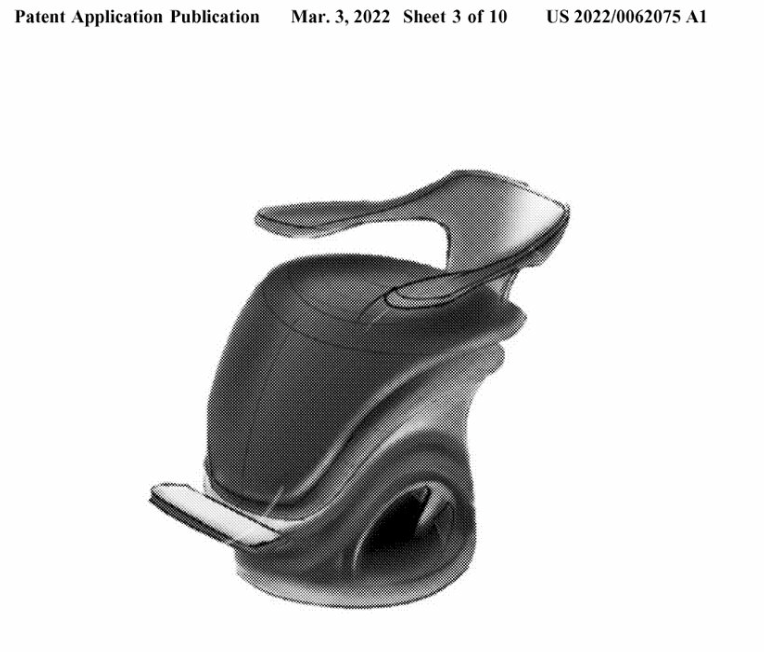
\includegraphics[width=0.6\textwidth]{US2022_0062075A1_Patent1.png}
    \caption{Patent US2022/0062075 A1: Hands-free wheelchair control system}
    \label{fig:patent1}
\end{figure}

Patent US2022/0062075 A1 (Fig. \ref{fig:patent1}) describes a hands-free control system but relies on head movements, which can be unintuitive and fatigue-inducing.

\begin{figure}[H]
    \centering
    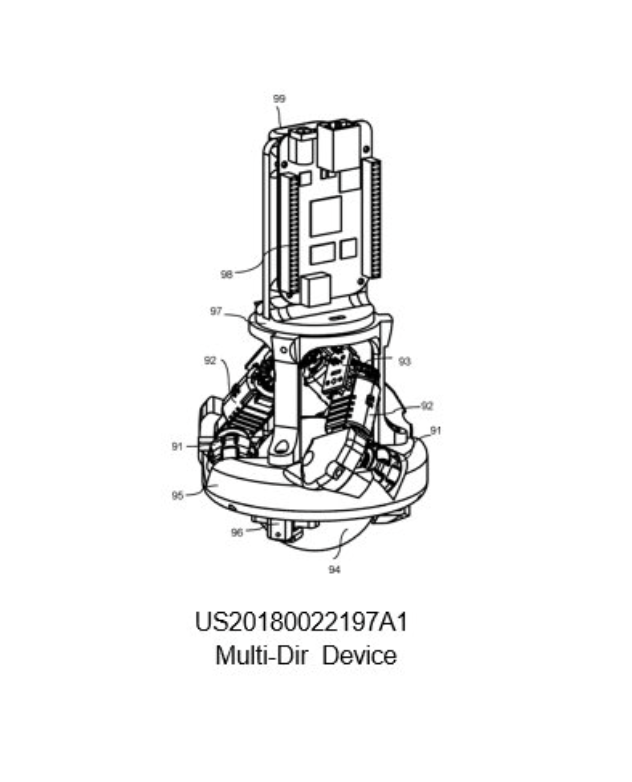
\includegraphics[width=0.6\textwidth]{US20180022197A1_Patent2.png}
    \caption{Patent US2018/0022197 A1: Omni-directional motion platform}
    \label{fig:patent2}
\end{figure}

Patent US2018/0022197 A1 (Fig. \ref{fig:patent2}) details an omni-directional platform. While relevant for movement, it lacks the integrated lean-control mechanism required for our specific sports application.

\subsection{Alternate Design Concepts}
Several design architectures were considered to achieve the hands-free, omni-directional goals.

\subsubsection{Concept 1: Segway-Style Self-Balancing Platform}
\begin{figure}[H]
    \centering
    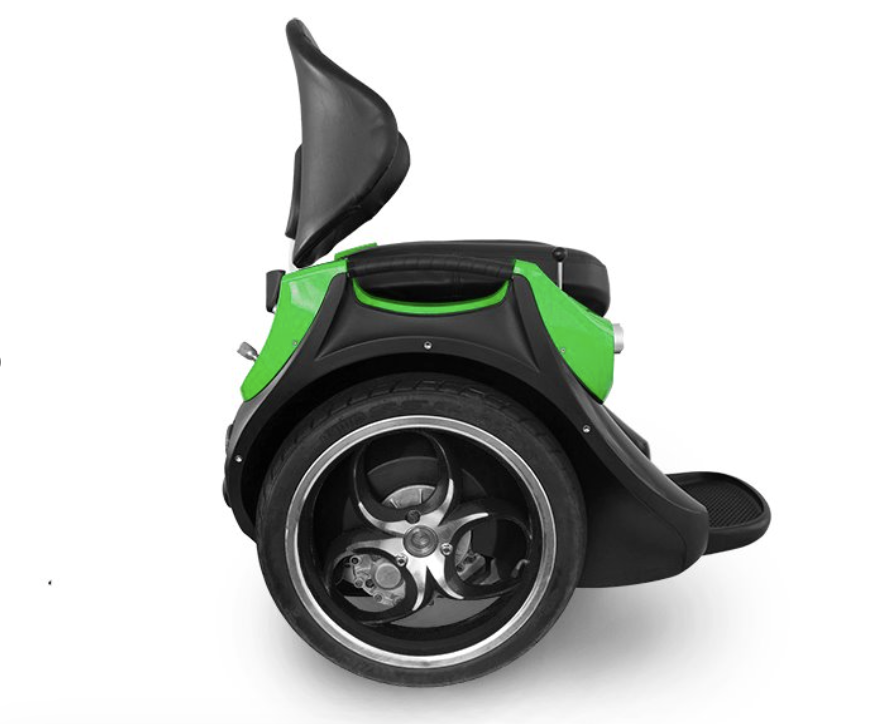
\includegraphics[width=0.6\textwidth]{Alt2Segway.png}
    \caption{Segway-Style Self-Balancing Concept}
    \label{fig:segway}
\end{figure}
This concept uses a two-wheeled self-balancing base. While intuitive for forward/backward motion, it lacks true omni-directional capability (sideways sliding) without complex additional mechanics.

\subsubsection{Concept 2: Mecanum Wheel System}
\begin{figure}[H]
    \centering
    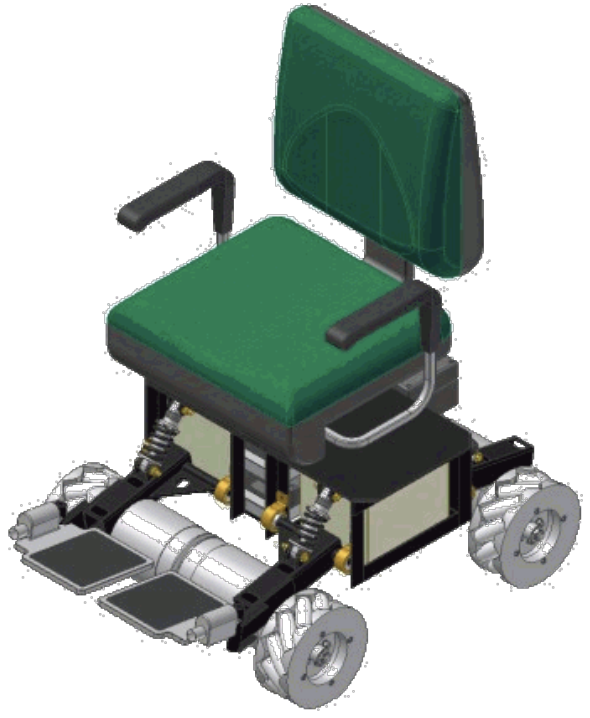
\includegraphics[width=0.6\textwidth]{Alt3Mecanum.png}
    \caption{Mecanum Wheel Concept}
    \label{fig:mecanum}
\end{figure}
A four-wheel Mecanum drive allows for translation in any direction. However, it requires a flat, consistent surface and does not inherently offer the intuitive "lean-to-move" feedback of a balancing system without complex software abstraction.

\subsubsection{Concept 3: Track-Based System}
\begin{figure}[H]
    \centering
    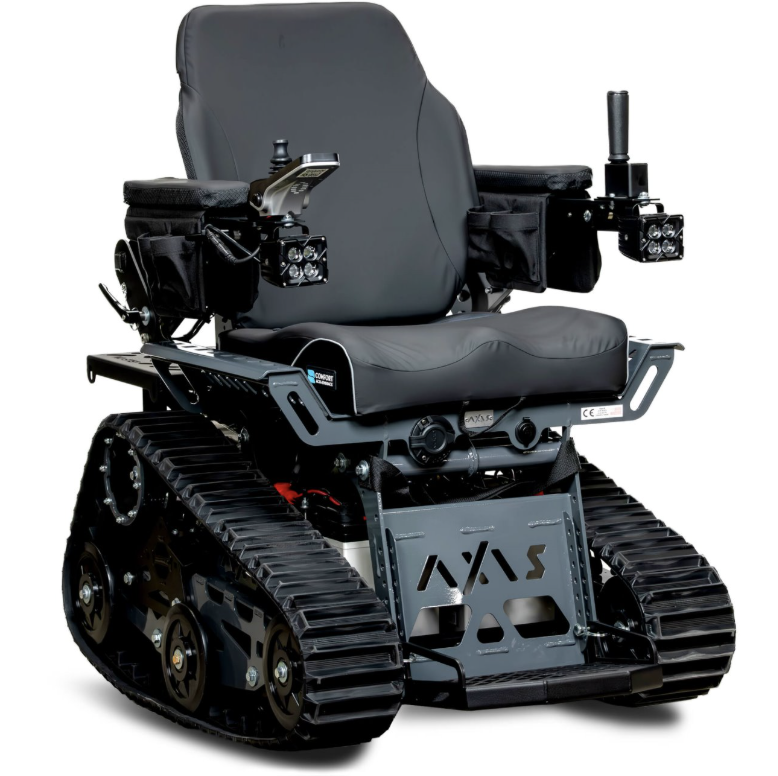
\includegraphics[width=0.6\textwidth]{Alt4Track.png}
    \caption{Track-Based Concept}
    \label{fig:track}
\end{figure}
A tracked system offers superior traction but is heavy, complex to steer omni-directionally, and has high friction, reducing efficiency for a battery-operated sports device.

\subsection{Design Selection Rationale}
The "Inverted Pendulum" Sphere Drive was selected as the optimal solution.
\begin{itemize}
    \item \textbf{Intuitive Control}: Unlike the Mecanum or Track systems, the sphere drive's balancing nature directly maps body lean to acceleration, mimicking natural walking/running dynamics.
    \item \textbf{Agility}: It offers superior omni-directional agility compared to the Segway (2-wheel) concept.
    \item \textbf{Simplicity}: It avoids the complex steering linkages of track systems.
\end{itemize}
This approach directly addresses the core need for hands-free operation while maximizing agility for basketball.

\section{Detailed Design \& Analysis}

The project's complexity is managed by breaking it down into three core engineering domains: Mechanical, Electrical, and Control.

\subsection{Mechanical Design}
Every advanced robot begins with a robust physical foundation. The mechanical design focuses on structure, agility, and safety.

\begin{figure}[H]
    \centering
    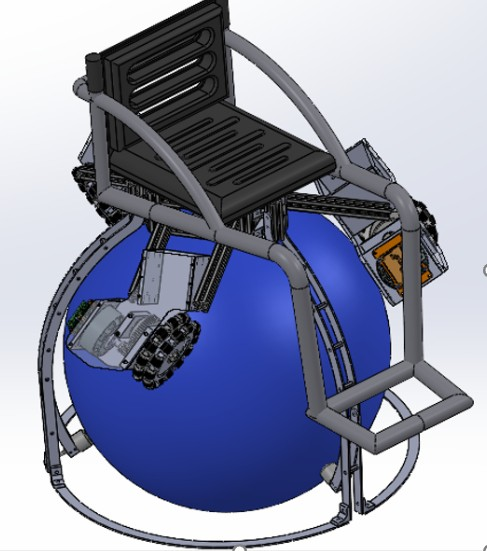
\includegraphics[width=0.8\textwidth]{fullDesign.jpg}
    \caption{Full Design of the Hands-Free Wheelchair}
    \label{fig:fulldesign}
\end{figure}

\subsubsection{The Sphere Drive System}
The wheelchair’s agility is achieved through a unique drive mechanism: a large, central sphere propelled by three precisely placed omni-wheels. Omni-wheels are special wheels with rollers that allow them to slide sideways while providing forward grip. This configuration allows the wheelchair to:
\begin{itemize}
    \item \textbf{Translate}: Move in any direction (forward, backward, sideways).
    \item \textbf{Rotate}: Spin on the spot.
\end{itemize}
This mimics the fluid, 360-degree agility of an able-bodied athlete.

\subsubsection{Solving the Grip Problem}
A critical challenge was the low friction between the polyethylene sphere and polyurethane rollers. The solution was to coat the sphere with SBR (Styrene-Butadiene Rubber) sheeting cut into a pattern of hexagons and pentagons, similar to a soccer ball. This ensures a reliable, no-slip grip.

\subsubsection{Key Structural Features}
\begin{itemize}
    \item \textbf{Adapted Chassis}: The core frame is adapted from a standard basketball wheelchair for familiarity.
    \item \textbf{Transmission}: Spur gears transfer power from motors to omni-wheels efficiently.
    \item \textbf{Tilt Limiter}: A passive mechanical "Safety ring" limits the platform's maximum tilt to 15 degrees, preventing tipping.
\end{itemize}

\subsection{Electrical System}
The electrical system manages power distribution, sensing, and motor drive. Given the rigorous demands of the "inverted pendulum" control capability, component selection prioritized low-latency communication and processing headroom.

\subsubsection{Key Components}
\begin{figure}[H]
    \centering
    \begin{subfigure}[b]{0.45\textwidth}
        \centering
        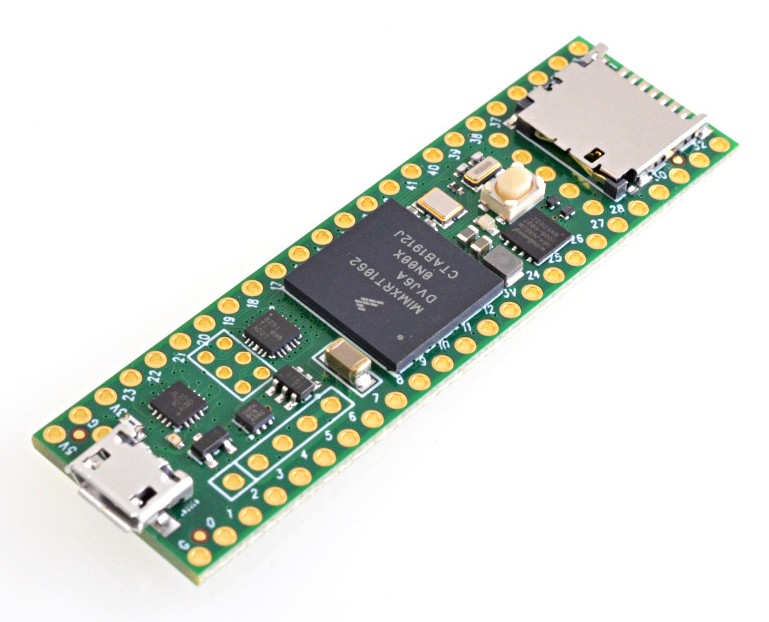
\includegraphics[width=\textwidth]{teensy.jpg}
        \caption{Teensy 4.1 Microcontroller}
        \label{fig:teensy}
    \end{subfigure}
    \hfill
    \begin{subfigure}[b]{0.45\textwidth}
        \centering
        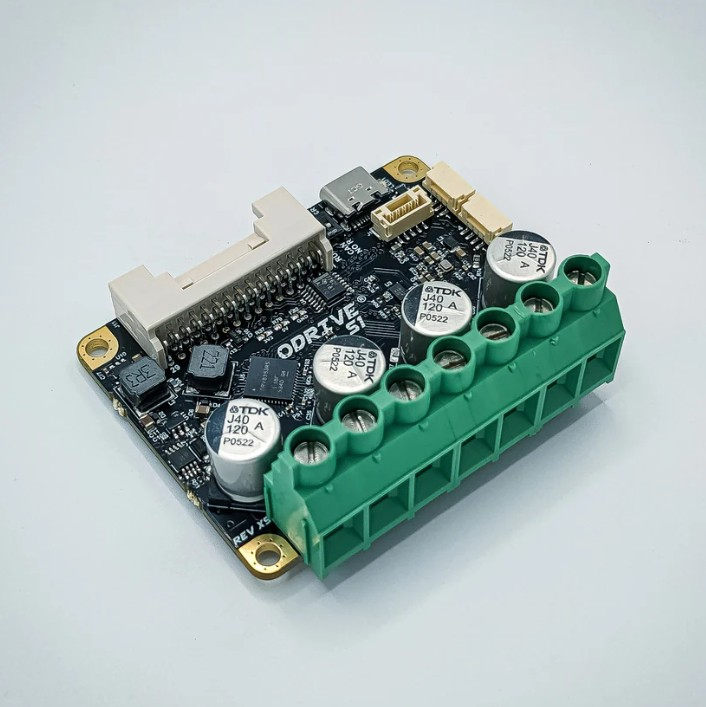
\includegraphics[width=\textwidth]{motor_controller.jpg}
        \caption{ODrive S1 Motor Controller}
        \label{fig:odrive}
    \end{subfigure}
    \vskip\baselineskip
    \begin{subfigure}[b]{0.45\textwidth}
        \centering
        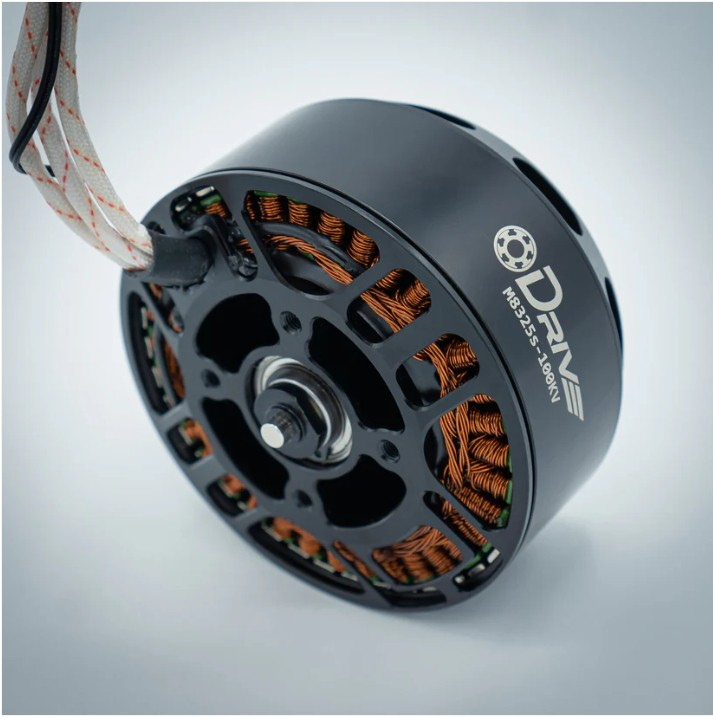
\includegraphics[width=\textwidth]{motor.jpg}
        \caption{M8325 Brushless Motor}
        \label{fig:motor}
    \end{subfigure}
    \hfill
    \begin{subfigure}[b]{0.45\textwidth}
        \centering
        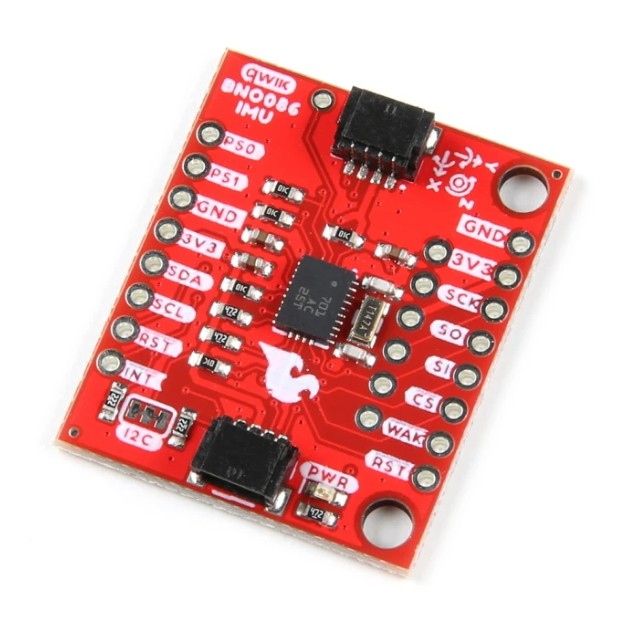
\includegraphics[width=\textwidth]{imu.jpg}
        \caption{BNO086 IMU Sensor}
        \label{fig:imu}
    \end{subfigure}
    \caption{Key Electrical Components}
    \label{fig:electrical_components}
\end{figure}

\subsubsection{Microcontroller Selection: Teensy 4.1}
The primary driver for this selection is the Teensy 4.1's superior handling of CAN communications compared to standard alternatives.

\paragraph{1. Native CAN Bus Architecture}
Unlike many standard development boards that require an external CAN controller (communicating via SPI, which introduces latency), the Teensy 4.1 features three internal CAN bus ports.
\begin{itemize}
    \item \textbf{Simplified Hardware Stack:} Because the CAN controller logic is embedded in the MCU, the hardware design only requires a simple CAN Transceiver (PHY) to interface with the bus. This reduces the Bill of Materials (BOM) complexity and failure points.
    \item \textbf{CAN FD Support:} The board supports CAN FD (Flexible Data-rate), which allows for higher bandwidth communication if our project requirements scale up in the future.
    \item \textbf{Library Support:} The hardware is supported by the highly optimized \texttt{FlexCAN\_T4} library, which supports asynchronous operation and FIFO buffering, ensuring no messages are dropped during high-load operations.
\end{itemize}

\paragraph{2. Ease of Implementation \& Development Velocity}
The Teensy 4.1 minimizes the friction often associated with high-performance embedded development.
\begin{itemize}
    \item \textbf{Ecosystem Compatibility:} It is fully compatible with the Arduino IDE via the Teensyduino add-on. This allows the team to utilize a familiar C++ environment without learning a proprietary vendor toolchain.
    \item \textbf{Rapid Prototyping:} The board's form factor (DIP-48) is breadboard-friendly for initial testing but robust enough to be soldered directly onto a carrier board or PCB for the final implementation.
    \item \textbf{USB Stack:} The Teensy features a robust USB stack that makes serial debugging, firmware uploading, and data logging to a PC significantly more reliable than standard serial adapters.
\end{itemize}

\paragraph{3. Robustness and Computational Headroom}
The project requires a controller that will not become a bottleneck as features are added.
\begin{itemize}
    \item \textbf{Processing Power:} Powered by an ARM Cortex-M7 running at 600 MHz, the Teensy 4.1 provides vastly more processing power than traditional 8-bit or 32-bit alternatives. This "over-provisioning" ensures that the CAN protocol handling does not interrupt or slow down other critical main-loop logic.
    \item \textbf{Memory Availability:} With 1024K RAM (512K tightly coupled), the system can handle large data buffers and complex state machines without running into the memory overflows common on smaller MCUs.
    \item \textbf{Reliability:} The NXP i.MX RT1060 processor used on the Teensy is an industrial-grade crossover processor designed for real-time applications, ensuring stable operation over long durations.
\end{itemize}

\subsubsection{Motor Controller Selection: ODrive S1}
The ODrive S1 was selected to function as a direct node on the CAN network managed by the Teensy 4.1.

\paragraph{1. Seamless CAN Bus Integration}
\begin{itemize}
    \item \textbf{Native CAN Interface:} The S1 supports CAN 2.0B at 1 Mbps, perfectly matching the native baud rate capabilities of the Teensy 4.1’s internal CAN controllers. This allows for a direct, high-speed command link without the overhead of USB or UART parsing.
    \item \textbf{Daisy-Chain Architecture:} The S1 features dual CAN connectors, allowing the three motors required for a ball bot to be daisy-chained. This significantly reduces wiring complexity and weight compared to a star topology.
    \item \textbf{Low-Latency Communication:} The simple binary CAN protocol minimizes bus traffic, allowing the Teensy to send torque commands at high frequencies ($>1$kHz) which is critical for the tight control loops required to maintain the ball bot's unstable equilibrium.
\end{itemize}

\paragraph{2. Critical Control Features for Balancing}
Balancing robots require specific control modes that standard hobby ESCs do not provide.
\begin{itemize}
    \item \textbf{Direct Torque Control:} The S1 provides precise direct torque control. In a ball bot, the IMU loop (running on the Teensy) calculates the necessary restorative force. The S1 allows the Teensy to command this force directly as current (Amps/Torque), bypassing velocity PID loops that would introduce phase lag and instability.
    \item \textbf{Field Oriented Control (FOC):} The S1 utilizes FOC to ensure that motor torque is smooth and silent, even at zero or low speeds. This is essential for a ball bot, which often hovers near zero RPM while balancing.
    \item \textbf{Regenerative Braking \& Brake Chopper:} Balancing involves constant acceleration and deceleration. The S1 includes an on-board brake chopper and connector for a brake resistor. This safely dissipates the energy generated when the robot decelerates to correct its lean, preventing bus over-voltage shutdowns that would cause the robot to fall.
\end{itemize}

\paragraph{3. Power Density and Mechanical Integration}
The S1 offers industrial-grade performance in a footprint suitable for a mobile robot.
\begin{itemize}
    \item \textbf{High Current Output:} Capable of 40A continuous and 80A peak current, the S1 provides the burst power necessary to recover from steep lean angles or external disturbances (kicks/pushes).
    \item \textbf{Compact Form Factor:} Measuring just 66mm x 50mm, it fits easily within the constrained chassis of a ball bot.
    \item \textbf{Locking Connectors:} The use of locking JST-GH and screw terminals ensures that connections remain secure despite the vibrations and shocks inherent in a balancing platform.
\end{itemize}

\subsubsection{Motors: M8325 High-Torque Brushless Outrunners}
The choice of the M8325 motor series is dictated by the unique physics of a direct-drive balancing platform.
\begin{itemize}
    \item \textbf{High Torque-to-Weight Ratio:} As an "outrunner" configuration, the M8325 generates significantly higher torque than in-runner equivalents. This allows for a gear-reduced setup that minimizes backlash—critical for balancing, where even millimetres of mechanical "slop" can cause oscillation and instability.
    \item \textbf{Thermal Mass for Stall Conditions:} Balancing robots frequently operate near zero RPM while holding high torque to keep the user upright. This "stall" condition generates significant heat ($I^2R$ losses). The large physical stator size of the 83mm motor acts as an effective heat sink, preventing thermal throttling during prolonged pauses in gameplay.
    \item \textbf{Low $K_v$ Design:} The selected winding rating (low RPM per Volt) is optimized for torque rather than top speed, ensuring the motors operate in their efficiency "sweet spot" during typical court maneuvers rather than requiring inefficient current-chopping at low speeds.
\end{itemize}

\subsubsection{Inertial Measurement Unit (IMU): BNO086}
The BNO086 was selected over standard sensors (like the MPU6050) because it provides "VR-grade" orientation data essential for human safety.
\begin{itemize}
    \item \textbf{On-Board Sensor Fusion:} Unlike basic IMUs that output raw acceleration and gyro data, the BNO086 features an internal Cortex-M0+ processor running proprietary fusion algorithms. It outputs corrected Quaternions directly. This offloads complex trigonometry and Kalman filtering from the main Teensy controller, freeing up cycles for the LQR control loop.
    \item \textbf{Drift Cancellation:} The sensor specifically addresses "gyro drift"—the tendency for yaw estimates to slowly rotate over time. Its internal magnetometer fusion ensures the wheelchair maintains a consistent "forward" heading down the court without requiring constant manual correction by the user.
    \item \textbf{Vibration Rejection:} Designed for virtual reality controllers, the BNO086 includes sophisticated filtering to ignore high-frequency mechanical vibrations from the chassis, ensuring the balancing algorithm reacts only to user lean and not road noise.
\end{itemize}

\subsubsection{Power Source: High-Discharge LiPo Batteries}
Lithium Polymer (LiPo) technology was chosen over Li-Ion (18650) or Lead-Acid due to the system's aggressive transient power demands.
\begin{itemize}
    \item \textbf{Handling Current Spikes:} The LQR controller may command virtually instantaneous direction changes to maintain balance, resulting in current spikes up to 80A. LiPo batteries offer high "C-ratings" (Discharge Rates) capable of delivering these bursts without significant voltage sag, which could otherwise reset the microcontrollers mid-game.
    \item \textbf{Voltage Stiffness:} The stability of the ODrive's bus voltage is directly correlated to motor performance. The low internal resistance of LiPo cells ensures that the voltage remains stiff even under load, providing consistent torque response regardless of battery percentage.
    \item \textbf{Form Factor Flexibility:} The pouch-style construction of LiPo batteries allows for a flatter, lower-profile pack. This aids the mechanical design by keeping the Center of Gravity (CoG) as low as possible, inherently improving the passive stability of the machine.
\end{itemize}

\subsubsection{Performance vs. Endurance}
To achieve the 4.5 m/s speed, high-torque motors were required. This resulted in a calculated 7.5-minute runtime, a trade-off prioritizing athletic performance over the initial 40-minute objective.

\subsection{System Integration and Implementation}
To translate our theoretical control model into physical motion, we implemented a distributed control architecture. This section details the wiring topology, the communication protocol, and the closed-loop logic used to achieve active balancing.

\subsubsection{Hardware Wiring Topology}
Our electrical implementation divides the system into two isolated voltage domains to prevent high-power motor noise from corrupting sensitive sensor data.

\paragraph{Low-Voltage Logic Domain (3.3V)}
The "brain" of the operation relies on 3.3V logic. We connected the components as follows:
\begin{itemize}
    \item \textbf{IMU Interface:} We interfaced the BNO086 IMU to the Teensy 4.1 via the I2C bus (Pins 18 SDA and 19 SCL). This link handles the high-speed transmission of orientation quaternions.
    \item \textbf{CAN Transceiver:} Because the Teensy outputs TTL logic, we integrated an SN65HVD230 transceiver. We connected the Transmit (CTX) and Receive (CRX) pins to the Teensy's hardware CAN1 port, allowing the microcontroller to interface with the differential signaling of the CAN bus.
\end{itemize}

\paragraph{High-Voltage Power Domain (24V)}
To power the motors, we utilized a "Star Topology" for power distribution but a "Daisy-Chain" for data.
\begin{itemize}
    \item \textbf{Power Distribution:} We routed power cables from the LiPo battery directly to each ODrive independently. This star configuration ensures that a high-current spike in Motor 1 does not cause a voltage sag that starves Motor 3.
    \item \textbf{Bus Termination:} To prevent signal reflection (echoes) on the communication lines, we installed a 120-Ohm termination resistor across the CAN High and CAN Low terminals of the final ODrive in the chain.
\end{itemize}

\subsubsection{Communication and Motor Addressing}
Since all three motors share the same two communication wires, we implemented a Node ID addressing system to differentiate them.

\paragraph{Physical Addressing}
We configured each ODrive S1 with a unique 6-bit Node ID using the on-board configuration switches/software:
\begin{itemize}
    \item \textbf{Axis 0 (Motor 1):} Node ID 0x0
    \item \textbf{Axis 1 (Motor 2):} Node ID 0x1
    \item \textbf{Axis 2 (Motor 3):} Node ID 0x2
\end{itemize}

\paragraph{The CAN Protocol}
We utilized the CAN 2.0B protocol running at 1 Mbps. This bandwidth allows us to send torque commands to all three motors in under 1 millisecond. The use of twisted-pair cabling for the CAN High and Low lines provides differential noise immunity, which is critical given the proximity of the wires to the high-magnetic-field motor coils.

\subsubsection{Control Loop Logic}
The system software runs a continuous loop on the Teensy 4.1, executing the following process every 2 milliseconds (500Hz):

\begin{enumerate}
    \item \textbf{State Estimation (Input):} The Teensy polls the BNO086 IMU via I2C to retrieve the current tilt angle ($\theta$) and tilt velocity ($\dot{\theta}$).
    \item \textbf{LQR Computation (Process):} We pass these state variables into our Linear-Quadratic Regulator (LQR) algorithm. The algorithm calculates the restorative torque required to zero out the error (i.e., return the robot to an upright position).
    \item \textbf{Kinematic Mixing:} The single "restorative torque" vector is split into three separate motor commands based on the geometry of the omni-wheels (120-degree separation).
    \item \textbf{Command Transmission (Output):} The Teensy packages these three torque values into standard CAN frames. For example, if the robot leans forward, the Teensy calculates the necessary counter-torque and sends a message to the specific motor responsible for that vector to spin in the opposite direction, thereby driving the wheels under the falling center of mass.
\end{enumerate}

\subsection{Control System}
The control system translates sensor data into motor commands.

\subsubsection{Linear-Quadratic Regulator (LQR)}
The team chose an LQR control method because:
\begin{itemize}
    \item It coordinates all three motors to control forward, sideways, and rotational movements simultaneously.
    \item It allows fine-tuning of the "feel" (responsiveness vs. smoothness).
    \item It provides a mathematical guarantee of stability.
\end{itemize}

\subsubsection{Simulation-First Workflow}
The controller was developed and tested in a MATLAB simulation before deployment. This allowed for safe testing of extreme maneuvers and rapid refinement without risking hardware.

\section{Project Management}

\subsection{Schedule and Project Timeline}
The project timeline is structured to ensure the systematic development, verification, and deployment of the hands-free wheelchair. The schedule is divided into four key phases as illustrated in the Gantt chart (Fig. \ref{fig:gantt}).

\begin{figure}[H]
    \centering
    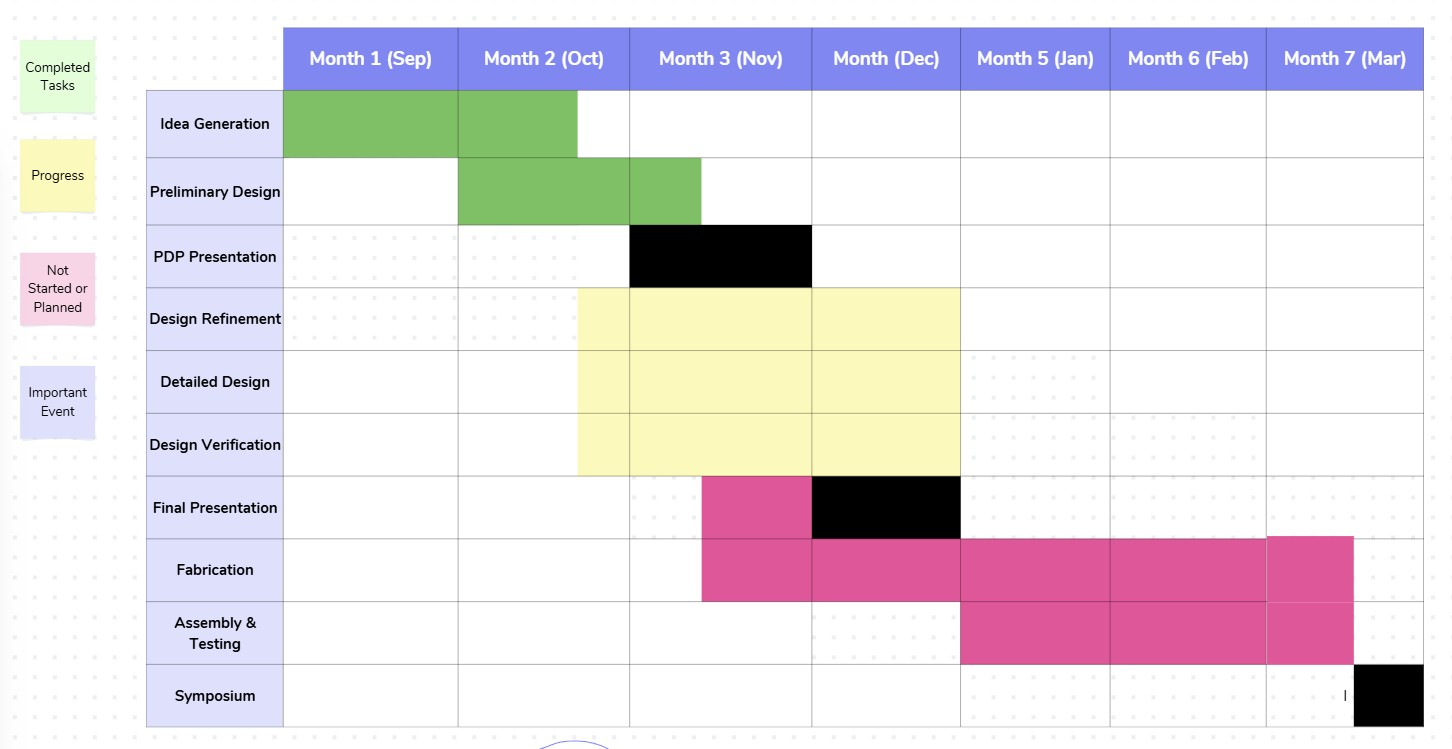
\includegraphics[width=0.9\textwidth]{GanntChart.jpg}
    \caption{Project Gantt Chart}
    \label{fig:gantt}
\end{figure}

\subsubsection{Phase 1: Conceptualization \& Preliminary Design (Completed)}
\textbf{September - November 2025}
This phase focused on defining the user needs and establishing the core "inverted pendulum" concept. Key achievements included:
\begin{itemize}
    \item \textbf{Idea Generation:} Brainstorming sessions to select the sphere drive architecture.
    \item \textbf{Preliminary Design:} Initial CAD modeling and component feasibility studies.
    \item \textbf{Milestone:} The Preliminary Design Presentation (PDP) was successfully delivered in November.
\end{itemize}

\subsubsection{Phase 2: Detailed Design \& Verification (Current)}
\textbf{November - December 2025}
The team is currently concluding this phase, which involves:
\begin{itemize}
    \item \textbf{Design Refinement:} Finalizing the mechanical chassis and electrical wiring topology.
    \item \textbf{Detailed Design:} Completing the LQR control simulations in MATLAB.
    \item \textbf{Design Verification:} Validating component choices (motors, batteries) against performance metrics.
    \item \textbf{Milestone:} This Final Design Report and the Final Presentation in December mark the end of this phase.
\end{itemize}

\subsubsection{Phase 3: Fabrication \& Assembly (Planned)}
\textbf{December 2025 - March 2026}
Following the final design approval, physical production will begin:
\begin{itemize}
    \item \textbf{Fabrication:} Manufacturing the T-slot aluminum chassis and 3D printing custom motor mounts.
    \item \textbf{Assembly:} Wiring the ODrive controllers and mounting the sphere drive system.
\end{itemize}

\subsubsection{Phase 4: Testing \& Validation (Future)}
\textbf{January - March 2026}
The final phase runs in parallel with the latter part of assembly:
\begin{itemize}
    \item \textbf{Commissioning:} Powering on the system and testing basic motor response.
    \item \textbf{System Tuning:} Calibrating the LQR controller on the physical hardware.
    \item \textbf{Milestone:} The project culminates in the Final Symposium in March, where the functional prototype will be demonstrated.
\end{itemize}

\section{Conclusions and Recommendations}

This project represents a sophisticated engineering effort to solve a real-world problem in accessible sports. The key design decisions—Sphere-Based Drive, Lean-Based LQR Control, and CAN Bus Architecture—create a system that is agile, intuitive, and robust.

We recommend continuing the development of the state estimation algorithms and conducting extensive user testing to refine the control sensitivity for different player styles.

\section{Teamwork Effort}
The team operated with a clear division of labor across the three pillars of design:
\begin{itemize}
    \item \textbf{Mechanical Team}: Focused on the chassis, sphere drive, and safety mechanisms.
    \item \textbf{Electrical Team}: Managed component selection, power distribution, and PCB design.
    \item \textbf{Control Team}: Developed the LQR algorithms and simulation environments.
\end{itemize}
Regular integration meetings ensured that mechanical constraints were communicated to the control team and that electrical requirements were met by the mechanical housing.

\section{Supporting Documents}

\subsection{Bill of Materials (Detailed Component Selection)}
The following table details the complete Bill of Materials (BOM) for the final design, including component costs and selection justifications.

\begin{longtable}{|p{0.2\textwidth}|p{0.25\textwidth}|c|r|p{0.3\textwidth}|}
\hline
\textbf{Component} & \textbf{Manufacturer / Part \#} & \textbf{Qty} & \textbf{Cost (CAD)} & \textbf{Description} \\ \hline
\endhead

\hline \multicolumn{5}{|r|}{{Continued on next page}} \\ \hline
\endfoot

\hline
\endlastfoot

IMU & Hillcrest Labs / Bosch BNO086 & 2 & \$108.76 & VR-grade IMU for high-precision orientation sensing. \\ \hline
CAN Transceiver & TI SN65HVD230DR & 1 & \$5.83 & Interface between Teensy TTL and CAN bus. \\ \hline
Microcontroller & PJRC Teensy 4.1 & 1 & \$54.94 & 600MHz ARM Cortex-M7 main controller. \\ \hline
LiPo Battery (6S) & Zeee 6S 22.2V 2200mAh & 3 & \$317.97 & High-discharge power source for wheel modules. \\ \hline
Motor Kit & ODrive S1 + M8325s & 3 & \$1,323.90 & Integrated FOC controller and high-torque motor. \\ \hline
Relay Switch & Hamolar 12V DC 120A & 2 & \$60.08 & High-current starter relay for safety switching. \\ \hline
Fuse Holder & BOJACK 100A ANL & 3 & \$47.97 & Circuit protection for high-current lines. \\ \hline
E-Stop Button & Yziixi 12-220V 3A & 1 & \$22.59 & Emergency stop for immediate system shutdown. \\ \hline
Walking Globe & Play Juggling 60cm & 1 & \$332.48 & 60cm Sphere for the main drive element. \\ \hline
Voltage Display & Agatige DC 100V 100A & 3 & \$39.57 & Real-time battery voltage monitoring. \\ \hline
Li-Ion Battery (7.4V) & YGHAPORT 2500mAh & 1 & \$17.49 & Logic power supply. \\ \hline
LiPo Battery (4S) & SIGP 14.8V 2250mAh & 1 & \$29.99 & Auxiliary power. \\ \hline
XT60 Parallel Cable & FLY RC & 3 & \$41.97 & Power distribution cabling (Parallel). \\ \hline
XT60 Series Cable & FLY RC & 3 & \$35.97 & Power distribution cabling (Series). \\ \hline
\textbf{Total Estimated Cost} & & & \textbf{\$2,439.51} & \\ \hline
\end{longtable}

\end{document}

